\documentclass[conference]{IEEEtran}
\IEEEoverridecommandlockouts
% The preceding line is only needed to identify funding in the first footnote. If that is unneeded, please comment it out.
\usepackage{cite}
\usepackage{amsmath,amssymb,amsfonts}
\usepackage{algorithmic}
\usepackage{graphicx}
\usepackage{textcomp}
\usepackage{xcolor}
\def\BibTeX{{\rm B\kern-.05em{\sc i\kern-.025em b}\kern-.08em
    T\kern-.1667em\lower.7ex\hbox{E}\kern-.125emX}}
\begin{document}

\title{Term Project Part-1\\
{\footnotesize }
}

\author{\IEEEauthorblockN{Abdullah Mert Tuncay}
\IEEEauthorblockA{\textit{Departmen of Computer Engineering} \\
\textit{Middle East Technical University}\\
Ankara, Turkey \\
2099422 \\
e2099422@ceng.metu.edu.tr}
\and
\IEEEauthorblockN{Baris Sugur}
\IEEEauthorblockA{\textit{Departmen of Computer Engineering} \\
\textit{Middle East Technical University}\\
Ankara, Turkey \\
2099315 \\
e2099315@ceng.metu.edu.tr}
}

\maketitle


\section{Introduction}
According to given topology from the Term Project, we designed a simple network which consists of 5 different nodes. In this document, we will start with the explanation of our design and how we implemented it. Then, we will share our experimental results about the implementation to show how our network behave in different manners. At the end, we share our experiences and comments about these parts of the projects.

\section{Design Approach}

\subsection{Understanding of the Topology}

According to the given topology, we are given 5 different nodes to construct a network. Each node has its special tasks which will be given by us according to our design. Starting with the source node, we stated that node as our client node and destination node as our server node. After that, we went on to the other nodes which are broker and routers. These nodes have individually different tasks since they have links to the both client and server sides. Starting with the broker, it has the most special tasks in design because it is acting like a converter in TCP and UDP part of the project. As stated in the topology we have a link which uses TCP between source and broker. On the other side, links between broker-routers and routers-destination uses UDP connection. Since broker has links for both sides, it needs to include sockets for both sides.

\subsection{Socket Programming Part}

After understanding how the nodes reacting each other, we focused on how we construct this links in our design. We simply meet socket programming which is the main approach for constructing this type of networks. According to socket programming, we have two type of nodes client and server. But in our topology as I mentioned above, we have different nodes which acting like both. In source node, we have client which initiates the connection. According to socket programming, client needs to now the address and the port of the server which will be the node that receives data or message. It's socket named as active socket. While moving onto the other nodes, we think other nodes as both client and server node(excluding the destination node) because these nodes both initiates the connection and wait  and respond for the clients. With this thought, we opens two sockets for the broker node. One node uses a socket with TCP connection to wait and respond the requests from the source node. On the other hand, second node uses 2 sockets with UDP connection to connect r1 and r2 routers. At the end, r1-destination and r2-destination uses UDP sockets,too.

\subsection{TCP vs UDP Sockets}
While designing the TCP and UDP sockets, we acknowledge some differences and we follow and implement according to it.In TCP, when a TCP client send data to the server, it requires an acknowledgement in return. If an acknowledgement is not received, TCP automatically retransmit the data and waits for a longer period of time. In UDP, the client does not establish a connection with the server. Instead, the client just sends a datagram to the server with requiring the address of the destination. Similarly, the server does not accept a connection from a client. Instead, the server just waits until data arrives from some client. At the end, the IP address of the client and the datagram is received, so the server can send a response to the client using these. We do not send big messages at the beginning so we cannot experience the message limit of two protocols. But according to researches, UDP datagrams are characterized by a length while TCP is a byte-stream protocol, which do not have any boundaries.

\subsection{Message}

For the beginning of our design, we use a simply a string to see the message is flowing through the nodes and arrive the destination node. After we accomplish our task, we divide string to two parts to send it from different routers. After doing that, because of using UDP which waits data to arrive, sometimes the sent string comes in different order and merges. After seeing that, we decide to send strings according to their sizes. At the end, we change the message to send the time we receive while in the source so it can be easy for us to calculate end-to-end delay. For future work, we try to send some strings which read from a .txt file and added the time beginning to it with a marker sign between them.


\section{Implementation Approach}

\subsection{Geni Platform and Programming Languages Choice}

At the beginning, we download the topology XML file to add resources in Geni platform. Then we use MAXI Insta Geni resources to go with. Then, we think about choosing Python which has an simple approach for handling socket programming. We examined the Python libraries according to our use and decided to choose it for our term project.
\subsection{General Features for Nodes}

For all node, there are several things that we do the same. Since we are using sockets to establish a connection between nodes, we kept HOST and PORT for the nodes. Excluding source nodes, all of our nodes consist multiple sockets since they have multiple links. At the broker node, we have 3 different sockets. One TCP socket for source node and 2 UDP socket for r1 and r2. Also, we use different ports for r1 and r2. For r1 and r2 node, we have two different sockets for destination and broker. At the end, for destination node we have 2 sockets for r1 and r2. Also their different port numbers included. In addition to these, we also construct a infinite loop to receive message and break(excluding source node).
\subsection{TCP Socket Implementation}

We construct a base client and server implementation for our TCP connection between source and broker. We opening a TCP socket with socket() function. Its parameters define the address family and socket type. Since TCP sends stream of data the term SOCK STREAM symbolize it. Also "AF INET" is Internet address family for IPv4. Then we connect the socket to server with server's hostname and port number used by the server. Then we send the all data with sendall(). At the server side, after we defining the socket, we bind the socket and make it listen to port until a connection received. Then we started a while loop, then accepted connection. From this connection, we received data and according to its length we send one of the routers using UDP links by using sendto().

\subsection{Broker Implemtation}

In broker implementation, we are having 1 TCP socket and 2 UDP sockets. After the definition of the HOST and PORT(which is the same for all nodes), we constructing a two sending sockets. These sockets are used to make a link between the routers and broker. After the UDP sockets are defined, we are constructing our TCP sockets to receive data. In this part, broker act like a server and bind to HOST and PORT and starting to listen to sockets for upcoming connection. Then inside an infinite loop, the connection was made and using the connection con we received the data. This infinite loop also terminate if the data is not received after the connection. After that the length of the message is calculated and the message is dividing into two. If it is length is even than it send message to r1 otherwise it send it to the r2. Since it is our choice to decide how to choose the routers in this part. We think this simple solution.

\subsection{UDP Socket Implementation}

In the broker, we initialize our first UDP sockets. The term SOCK DGRAM is telling us about the sockets that this socket will use UDP connection. We defined 2 send sockets for our 2 different routers r1 and r2. Then send the data according to the message lengths. The operation in r1 and r2 is the same since their tasks is same. We defined a new send socket and one socket to bind for the coming data from the broker. Then receive data and send it to the destination by using sendto(). In these UDP links, we do not ever need to make a connection or listen to it. We just bind to the related host and port and wait for receiving the data. In destination implementation, constructing a socks array to saved binding sockets in it. Then in our infinite loop, we construct a for loop for each of the sockets to receive message. 

\subsection{End-to-End Delay Calculation}

In our project, we experience that the local time of the nodes may be differ in seconds. So we calculate end-to-end delay by using the message we sent. We use an external library named ntplib for python.(To install : pip install ntplib) With using ntplib, we are making a request to "time.google.com" and saving that request in a variable. Then using datetime library we save the time from the google in a detailed way (consisting msec). Then we converted it to string and then using encode() function we can convert it to byte. After all of these operations, the leaving time of message is saved and sent through the port. We are using print statement in several places to control the change in time. At the end, after we receive the data in destination, we calculate the time of arrival by using the same method we used in source and find their difference to calculate end-to-end delay.

\section{Experimental Results}
Below there are four graphs that relates to tc/netem delays vs end-to-end delay. We thought the best way to compare these result to first try without and delays. (Only with natural connection delays.) We also plot a graph for it. 


\subsection{No Delay}

Below is the graph that sends the message without any tc/netem delays. From this graph, we will compare the end-to-end time change when different delays are added.

\begin{figure}[h]
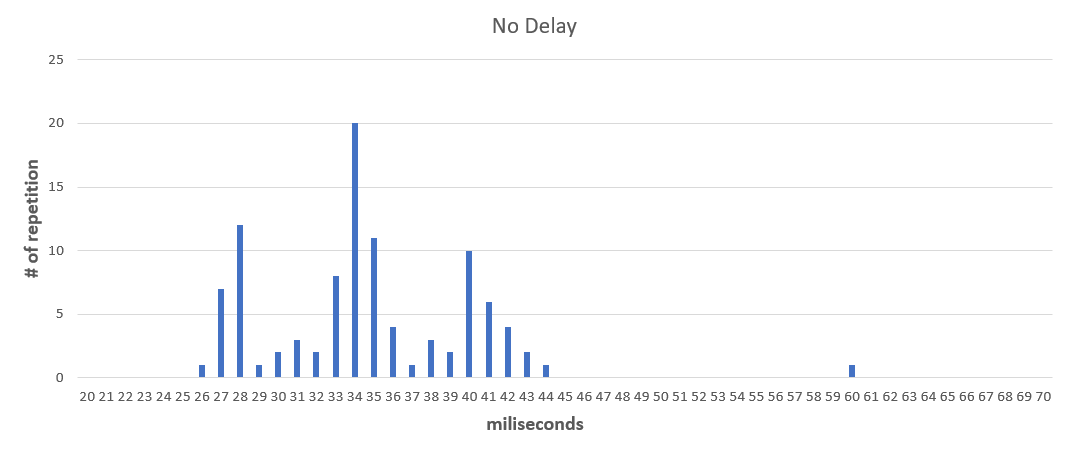
\includegraphics[width=0.45\textwidth]{No_Delay.png}
\caption{No Delay Added}
\label{fig:figure2}
\end{figure}
Sample size: 100 \\
Mean: 35.1 ms \\
Standard deviation: 5.3 ms \\
For this graph, both our connection and nodes connections was a bit ambiguous, so the graph didn't turned out to be a perfect but it still make sense. The \%95 confidence interval can be calculated with the following formula:

$$X \pm Z \dfrac{s}{\sqrt{n}}$$
Where; \\
X = mean \\
Z = 1.96 (for \%95 confidence interval) \\
s = standard deviation \\
n = sample size \\
Hence, for this graph, the confidence interval is:
$$35.1 \pm 1.96 \dfrac{5.3}{\sqrt{100}} = 35.1 \pm 1.04ms$$

\subsection{1ms Delay}

\begin{figure}[h]
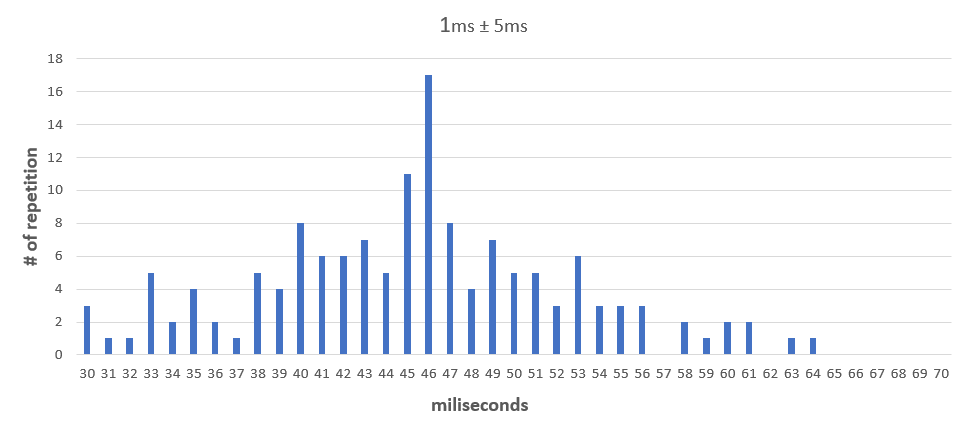
\includegraphics[width=0.45\textwidth]{1_ms.png}
\caption{1 ms Delay Added}
\label{fig:figure2}
\end{figure}
Above is the tc/netem delay vs end-to-end time graph that sends the signal with $1ms \pm 5ms$ delay. \\
Sample size: 144 \\
Mean: 45.3 ms \\
Standard deviation: 7.7 ms \\
For this graph, the confidence interval is:
$$45.3 \pm 1.96 \dfrac{7.7}{\sqrt{144}} = 45.3 \pm 1.26ms $$
Notice that the end-to-end delay is increased from 35-36 to 44. This was a bit higher than we expected since the increase should have happened around 3-4 ms but still this graph make sense because there is 5ms noise and  end-to-end time is increased compared to the graph before any delay happened.

\subsection{20ms Delay}

\begin{figure}[h]
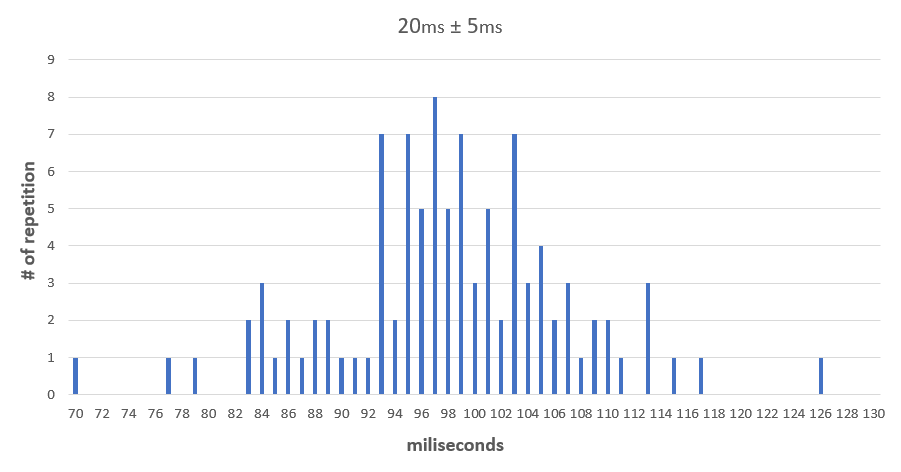
\includegraphics[width=0.45\textwidth]{20_ms.png}
\caption{20 ms Delay Added}
\label{fig:figure2}
\end{figure}
Above is the tc/netem delay vs end-to-end time graph that sends the signal with $20ms \pm 5ms$ delay. \\
Sample size: 102 \\
Mean: 99.2 ms \\
Standard deviation: 10.6 ms \\
For this graph, the confidence interval is:
$$99.2 \pm 1.96 \dfrac{10.6}{\sqrt{102}} = 99.2 \pm 2.06ms$$
This graph make much more sense and probably the best graph we get because it is indeed looks like a binomial distribution graph and the mean end-to-end delay is nearly perfect. Since each node has 20ms delay, we expected 60 $\pm$ 15 delay on top of the delay we measured without any tc/netem delay. (Which is aroud 96 $\pm$ 15ms). And we indeed get the nearly exact result.
\subsection{60ms Delay}

\begin{figure}[h]
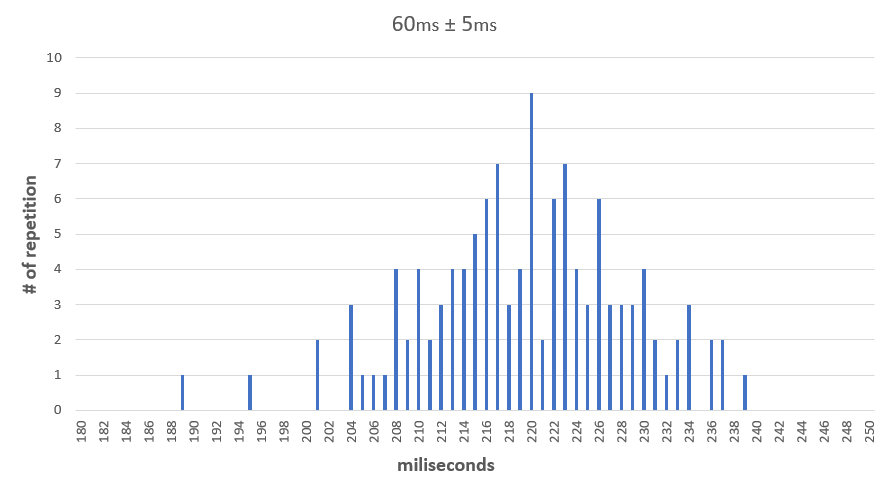
\includegraphics[width=0.45\textwidth]{ms.png}
\caption{60 ms Delay Added}
\label{fig:figure2}
\end{figure}
Above is the tc/netem delay vs end-to-end time graph that sends the signal with $60ms \pm 5ms$ delay. \\
Sample size: 121 \\
Mean: 220.4ms \\
Standard deviation: 9.8 ms \\
For this graph, the confidence interval is:
$$220.4 \pm 1.96 \dfrac{9.8}{\sqrt{121}} = 220 \pm 1.75ms$$ \\
We believe this is also a pretty good result. The expected result was 180 $\pm$ 15ms on top of the normal delay that calculates around 215 $\pm$ 15ms which is pretty close to our result.

\subsection{Conclusion of Experiment}
It is clear that tc/netem delays are changed the overall end-to-end delay. We have been able to calculate and get pretty close results, comparing with the non-delayed graph, tc/netem delayed graphs are much better results which may be caused by the fixed delays (1ms,20ms,60ms). 

\section*{Comments}

\subsection*{}
In the part-1 of the term-project, we happen to encounter many of the different problems and errors. Many of the related issues are related to the connection between our local machines and the connected ssh nodes. In ssh connection, due to the slowness of the ssh connection in the nodes, we are having trouble about changing so much of our codes. 

\subsection*{}
In the design part, we start to think as simple as possible to prevent complicated errors while constructing the topology we are given. After the simple implementation is finished, we focused on the main task about how we can change to do better or how we can do it faster. We wrote a script that changes all files in the nodes with the local ones. On the other hand, we focus on the message part first about how we can customize it to our needs. This shows us the difference between the message length or size limit difference in UDP and TCP. 

\subsection*{}
In conclusion, we have managed to create connections between the nodes and calculate the effect of tc/netem delays on the end-to-end delay. This project was very helpful for us to understand the connections and delays between hosts and servers.

\end{document}
